\begin{frame}
    \frametitle{Optical encoders}
    \scriptsize
    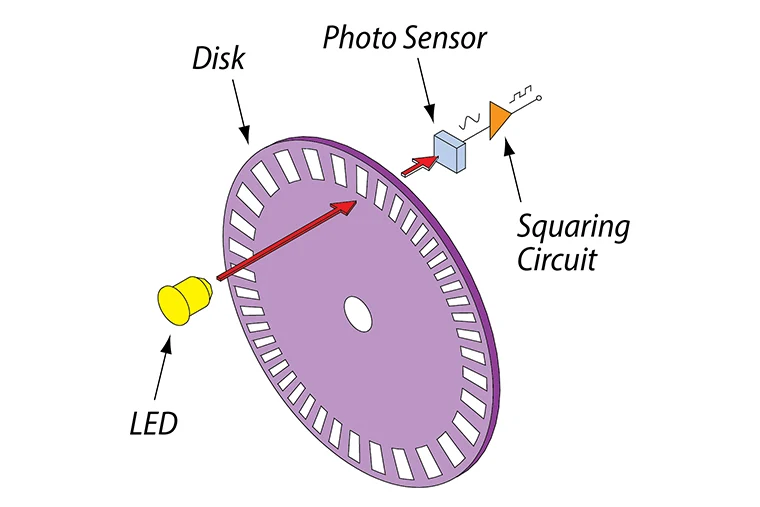
\includegraphics[width=0.45\columnwidth]{images/encoder_principle}
    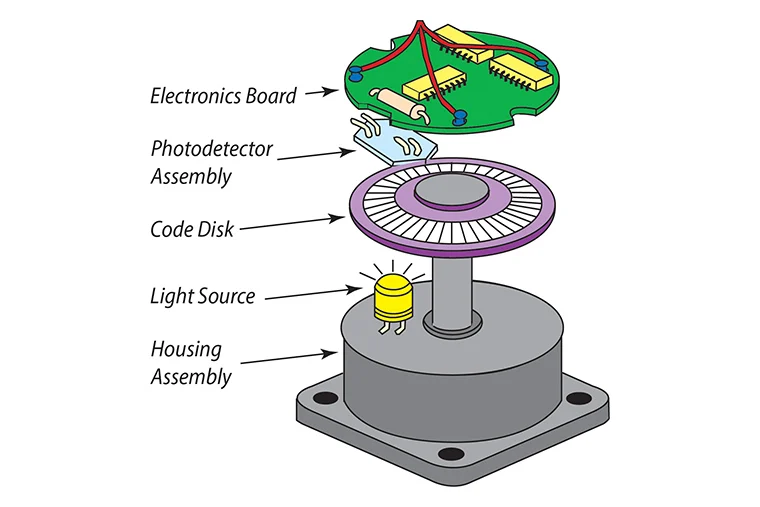
\includegraphics[width=0.46\columnwidth]{images/encoder_parts}
    \footnotesize

    \begin{block}{Principio de funcionamiento}
        %Consta de una fuente de iluminación un disco rotor con una fina rejilla óptica que gira con el eje y un detector ópticos fijo.
        A medida que el rotor se mueve, la cantidad de luz que incide en el detector óptico varía según pase o no la luz. La onda sinusoidal resultante se transforma en una onda cuadrada discreta utilizando un umbral para elegir entre estados claros y oscuros. %La \textbf{resolución} se mide en ciclos por revolución (CPR). La \textbf{resolución angular mínima} se puede calcular fácilmente a partir de la clasificación de CPR de un codificador. Un codificador típico en robótica móvil puede tener 2000 CPR.
    \end{block}
\end{frame}

\begin{frame}
    \frametitle{Optical encoders}

    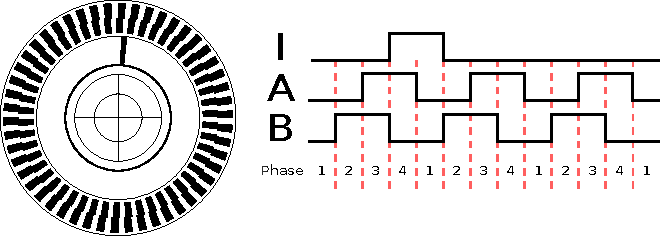
\includegraphics[width=\columnwidth]{images/encoder.pdf}
    \footnotesize

    La relación de fase observada entre los trenes de impulsos del canal A y B se utiliza para determinar la dirección de rotación. Una sola ranura en la pista interior genera un pulso de referencia (índice) por revolución.

    \begin{itemize}
        \item Proprioceptivo
        \item La resolución se mide en ciclos por revolución (CPR). Suelen tener 2000 CPR.
        \item La odometría basada en encoders acumula error rápidamente por diferencias físicas en en las ruedas, deslizamiento o giro en el aire de las ruedas.
    \end{itemize}
\end{frame}